\documentclass[../main.tex]{subfiles}
\begin{document}

\section{Experiment Scheme}\label{sec:experiment_scheme}
Our method of plasma generation is based on the laser trigger technique with the injection of gas (a mixture of \SI{95}{\percent} N\textsubscript{2} and \SI{5}{\percent} H\textsubscript{2}) inside the capillary \cite{Bobrova2002SimulationsWaveguide,Spence2001InvestigationWaveguide}.
The waveguide is designed to operate in an evacuated chamber, maintained at $\sim$\SI{e-4}{\torr}.
\begin{figure}
\centering
    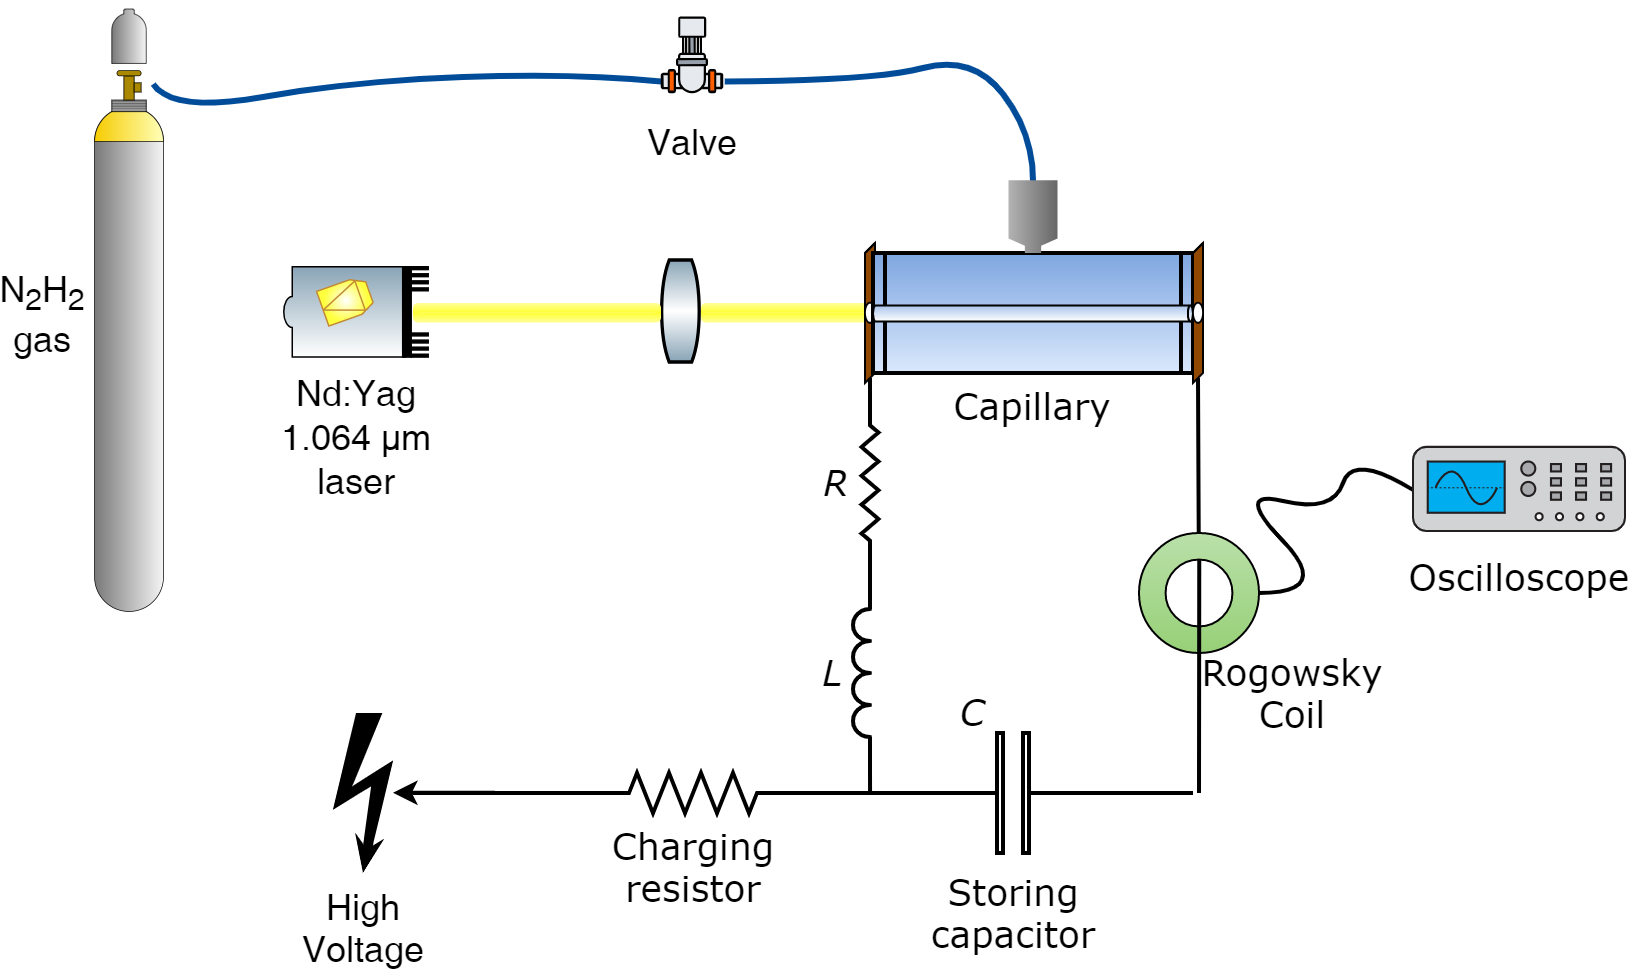
\includegraphics[width=\textwidth]{figures/Laser-based ignition scheme.png}
    \label{fig:scheme}
    \caption{Plasma generation in the N\textsubscript{2}+H\textsubscript{2} gas--filled capillary. The vacuum chamber has been omitted for clarity.}
    \end{figure}
The experimental system is shown in figure \ref{fig:scheme}, and applies to all forth--coming discussion.

Two electrodes are mounted at both ends of the capillary. Those electrodes are connected to a high-voltage source, which provides a pulse of a few kilovolts amplitude, during the opening of a valve\sidenote[][-50mm]{Product of \textit{Parker Hannifin Corporation}, model 099-0340-900}, set to be opened for \SI{30}{\ms}, that fills the the capillary with gas. The ignition is achieved by the igniting laser pulse, that ionizes matter and detaches electrons \cite{Palchan2007ElectronChannel}, which in turn accelerate under the applied high voltage and in an avalanche manner, plasma discharge manifests inside the capillary. The created electron current effectively closes an electrical circuit, for which the plasma ignition acts as a switch. The discharge current is recorded by a Rogowski coil \sidenote[][-75mm]{\textit{Pearson}, model 110A. A wide band current transformer with typical response time of less than \SI{50}{\ns}.} and the current profile is acquired by an oscilloscope.

\begin{marginfigure}[-60mm]
    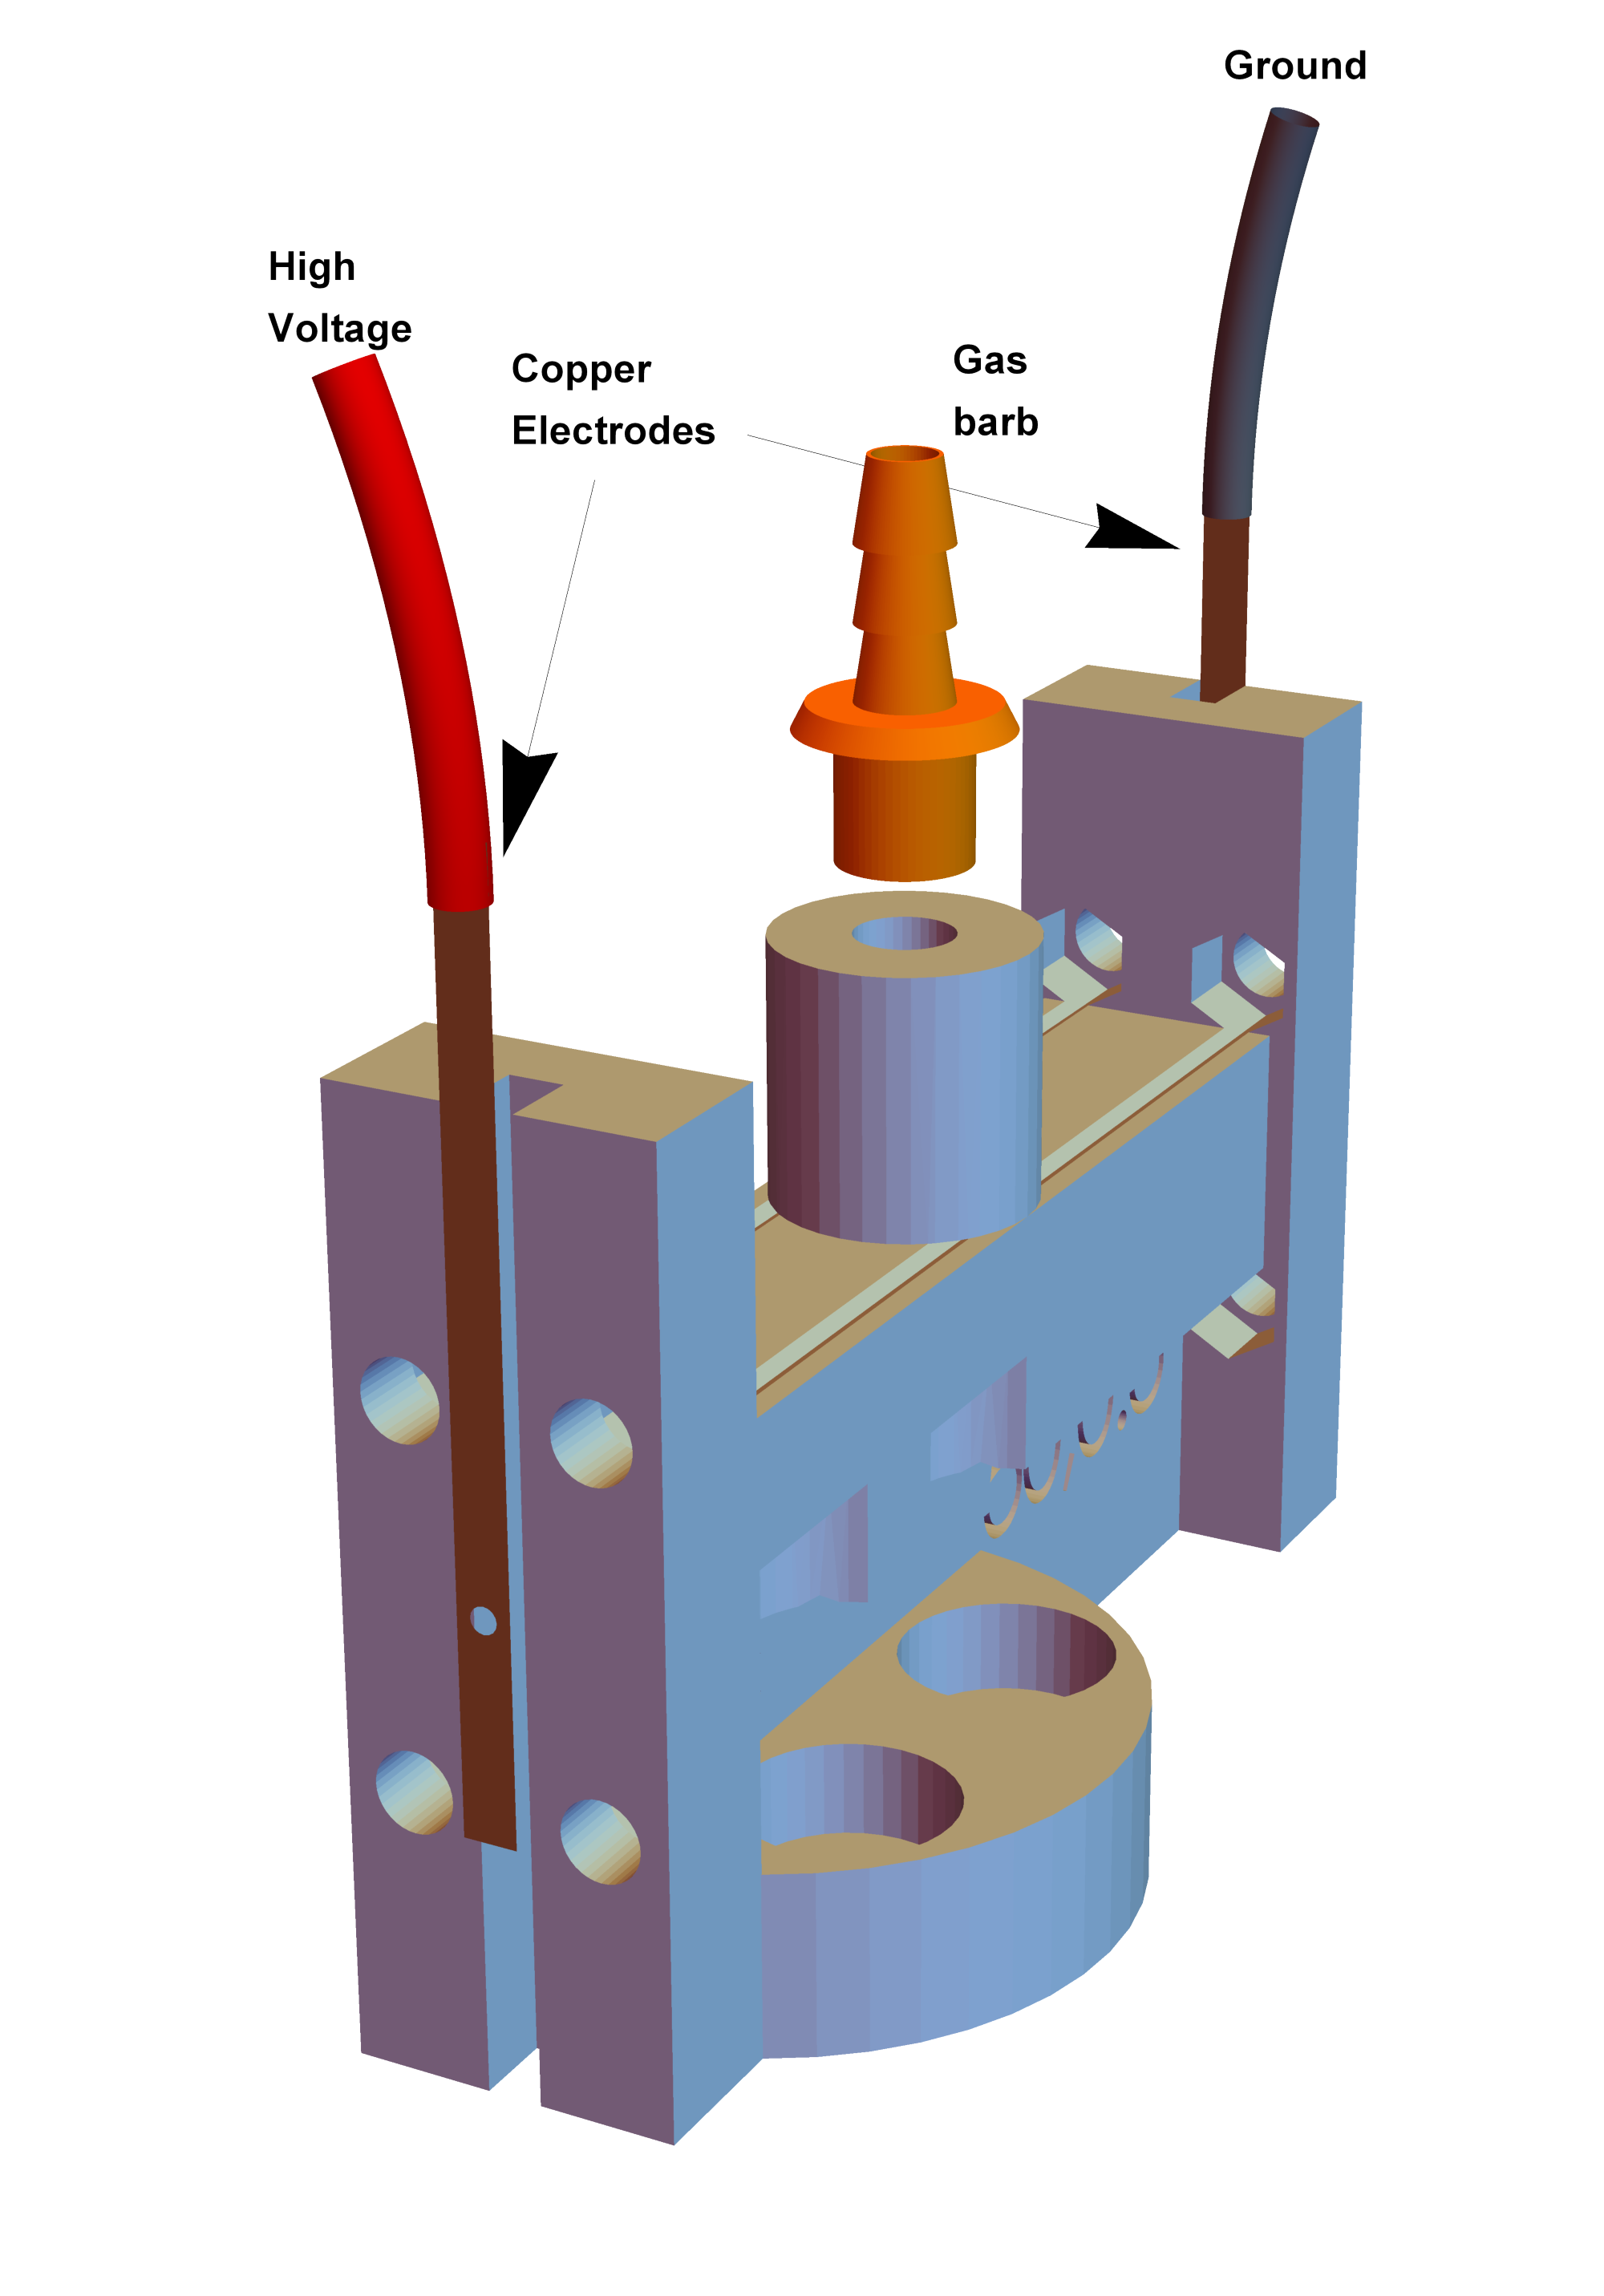
\includegraphics[width=\marginparwidth]{figures/cad/setup.pdf}
    \caption{The 3D printed capillary shown with the two electrodes and a hose--barb to inject the gas.}
    \label{fig:setup}
\end{marginfigure}

	\section{Devices in use}\label{sec:devices}
The experiment was conducted using the following devices:
\begin{enumerate}
    \item Capillary
    \item Nd:Yag Laser, 1064 nm
    \item Oscillator laser, 800 nm
    \item High Voltage power supply
    \item Spectrograph and Andor ccd camera
    \item Photodiodes
    \item Optical Elements, viz., lenses and mirrors
    \item Rogowsky coil
    \item Digital delay and pulse generator
    \item Gate valve
    \item Vacuum chamber
\end{enumerate}
\subsection{Capillary production}
The capillary is the medium at which the plasma channel forms. Its length is \SI{5}{\cm}, and its inner diameter is \SI{500}{\um}. The plastic unit is made of a photopolymer, created in a 3D printer, and is shown in figure \ref{fig:onecapillaryCAD}. A hose connects at the top circular extrusion in the upper face to fill the capillary with gas.
\begin{figure*}[b]
    \centering
    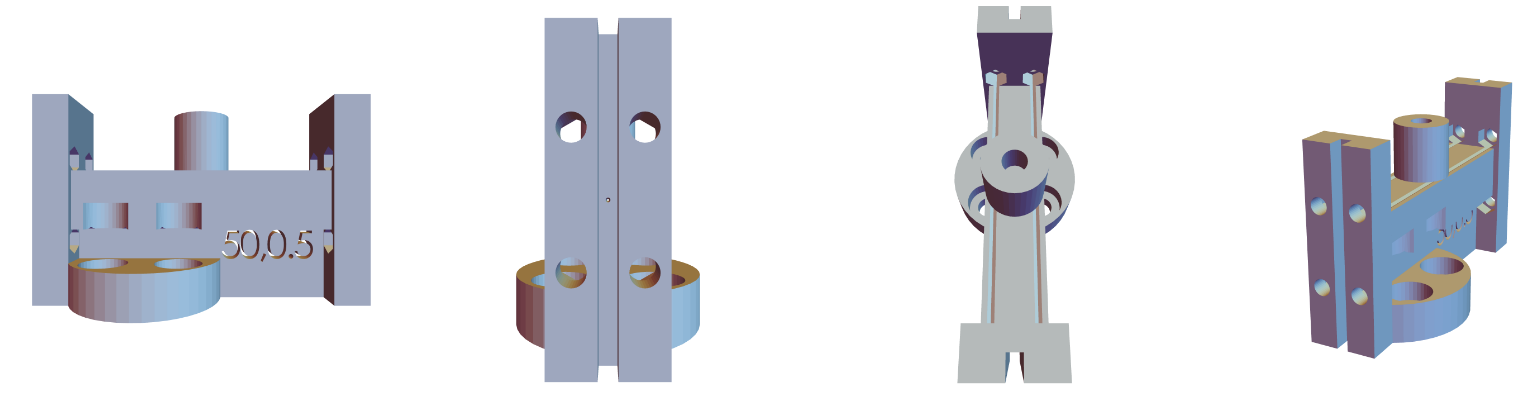
\includegraphics[width=\textwidth]{figures/cad/onecapillary_cad.PNG}
    \caption{3D drawing of the straight capillary.  Designed by Yair Ferber.}
    \label{fig:onecapillaryCAD}
\end{figure*}
\subsection{Lasers used}\label{ssec:lasers}
In our system two laser were in use, igniting laser and an oscillator laser:
\begin{itemize}
\item The first is \textit{Tempest 10}, a \SI{1.064}{\um} pulse laser, flashlamp pumped, Q-switched, Nd:Yag laser manufactured by \textit{New Wave Optics}. The pulse duration is $\tau \sim$ \SI{10}{\ns}, and with energy of up to $\sim$ \SI{200}{\mJ}. The ignition of the plasma is initiated by this laser pulse that ablates a small amount of surface in the inner wall of the capillary and produces seed ionization that triggers the discharge after $\sim$\SI{50}{\ns}. In the experiment the energy being used in most cases to obtain reliable ignition was $\sim$\SI{50}{\mJ}. The laser beam was delivered on the capillary axis through the negative electrode by a focusing lens.
\begin{marginfigure}
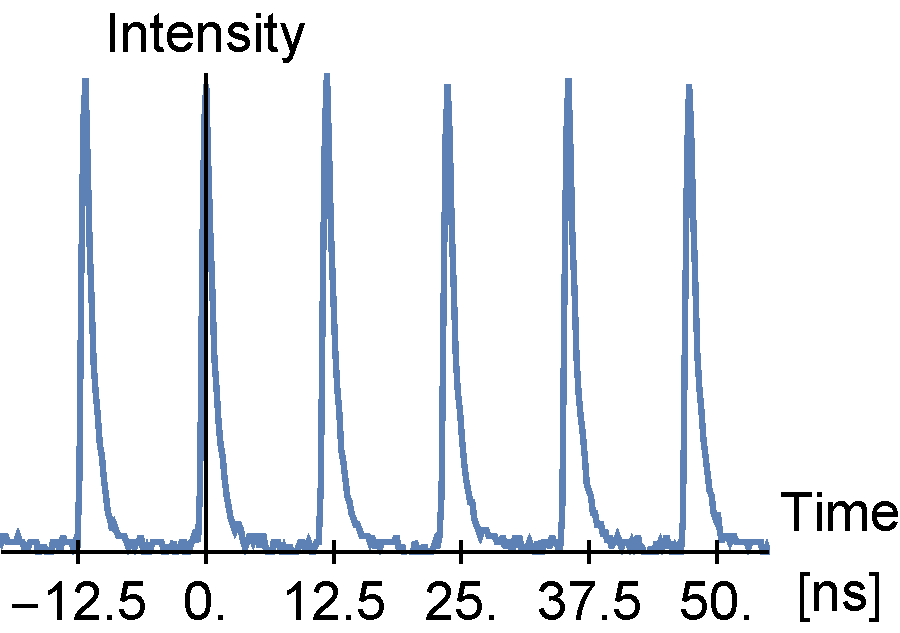
\includegraphics[width=\marginparwidth]{figures/oscillator/single.pdf}
\label{fig:oscillator_single}
\caption{Oscillator laser, \SI{84}{\MHz} temporal beam profile.}
\end{marginfigure}
\item The second laser is \textit{Mai Tai}, a \SI{800}{\nm} mode-locked oscillator, manufactured by \textit{Spectra Physics}, with a Ti:Sa crystal as the lasing medium.
It produces \SI{15}{\fs} temporal pulses at a \SI{84}{\MHz} rate (i.e., a pulse every \SI{12.5}{\ns}) with \SI{5}{\nano\J} per pulse. This beam was directed, in some parts of the experiment, through the capillary and recorded with a fast photo--diode\sidenote{\textit{ThorLabs DET10A}} (see figure \ref{fig:oscillator_single}), thus enabling one to compare the optical guiding at different times along the discharge process.
\end{itemize}
\subsection{High Voltage pulser}
The high voltage pulser provides the high voltage difference applied on the two electrodes. See picture on the right. Its key element is the energy storing capacitor that must be charged to a high voltage (that to be applied on the electrodes) and then discharged through the capillary and the rest of the electric chain. The pulser was designed, built, and still maintained, by Levin. See  \cite{Levin2009ExcitationAcceleration} pp. 46-47, for more information considering the setup and explanation of its operation.
\begin{marginfigure}
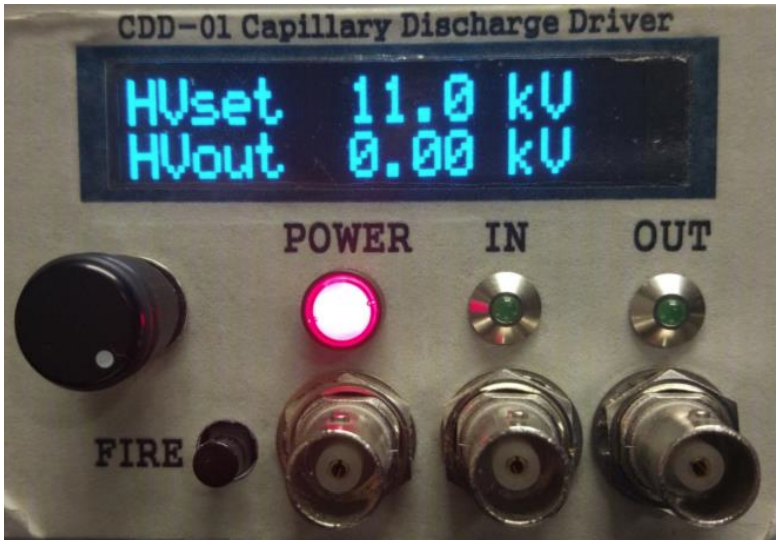
\includegraphics[width=\marginparwidth]{figures/hvpulser.PNG}
\caption{Discharge Pulser high voltage, designed, built and Maintained by Michael Levin.}
\end{marginfigure}
	
\subsection{Spectrograph and Andor CCD camera}\label{ssec:spectro}
To measure the capillary plasma density and to validate the existence of a hollow radial density profile at the time segment optical guiding exist, we performed a direct spectroscopic study of the plasma emission. The plasma emission during the discharge was collected by an imaging system and imaged onto the entrance slit of a detection system, composed of a spectrometric instrument\sidenote{\textit{Spectra--Pro} model 300i}, fitted with a 2D 1024$\times$256 element intensified charge-coupled device (CCD) fast camera\sidenote{\textit{Andor}, model DH520.}. The CCD allows for recording images with both spectral and spatial resolution.

The detector gating and delay were set by a digital delay and pulse generator\sidenote{\textit{Stanford Research Systems},\newline model DG--535.} that triggers the CCD camera.

The spectrometric instrument is a Czerny-Turner arrangement, made of a plane reflection grating. Light entering the entrance slit is collimated by a concave mirror and directed towards the plane reflection grating. Light diffracted from the grating forms a plane wave that is focused by another concave mirror onto the exit slit. Only one wavelength leaves the grating in the right direction to reach the exit slit, and tuning is achieved by rotating the grating, controlled by Andor's computer software. See figure \ref{fig:spectrometer}. In our measurements we used a 1800 lines/mm grating; Spatial resolution is controlled by the width of the entrance slit.
\begin{marginfigure}
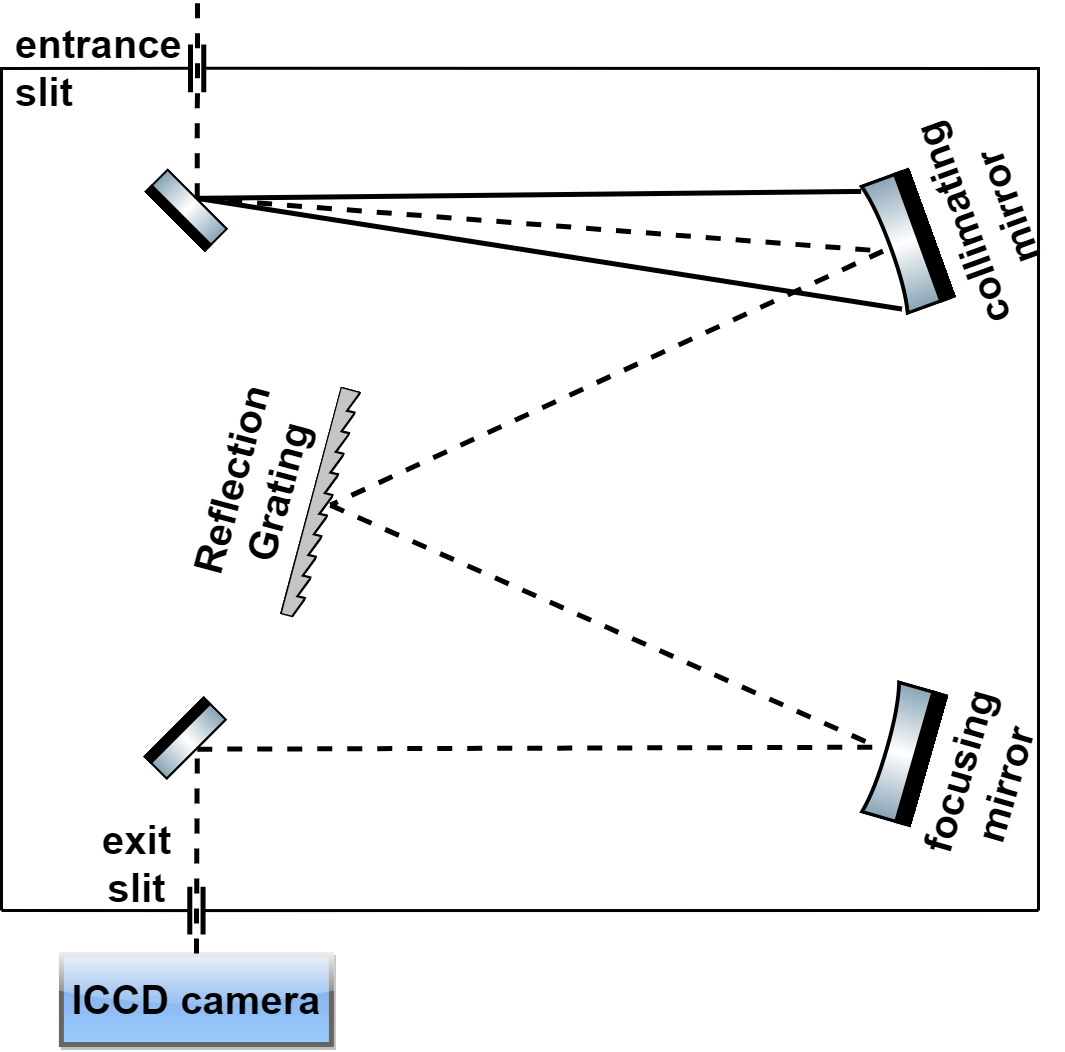
\includegraphics[width=\marginparwidth]{figures/spectro/spectrometer.png}
\caption{Optical layout for the spectrometric instrument.}
\label{fig:spectrometer}
\end{marginfigure}

\end{document}